
%================ch1======================================

\section{Introduction}\label{sec:introduction}
Agricultural intensification, mechanization, and automation have all led to major increases in agricultural productivity throughout time [2]. Robots are intelligent machines that may be trained to carry out particular jobs, make choices, and take immediate action. They are needed in a variety of industries, and they function best in stable environments where consistent accuracy and high productivity are required [3]. Robots have become increasingly important in today's companies as they offer a wide range of benefits, including increased efficiency, improved safety and reduced labor costs. With the fast pace of technological advancement, it is expected that robots will play an even greater role in companies in the future. Companies that invest in robots will be better able to compete in today's global economy, and will also be well positioned to take advantage of new opportunities as they arise.~\\

\noindent Another important aspect of robots in today's companies is their ability to be eco-friendly. Robotics technology has advanced to such a level that it is now possible to design robots that are energy-efficient and use sustainable materials. Additionally, many robots are designed to be lightweight and compact, which reduces their overall energy consumption and carbon footprint.

\noindent Moreover, robots can also be used in the field of agriculture and farming, where they can help to improve crop yields and reduce the need for pesticides and other chemicals. This can help to reduce the environmental impact of farming, while also increasing food production. As robots continue to evolve and become more advanced, it is important for companies to consider the environmental impact of their usage and take steps to make them as eco-friendly as possible. By doing so, they can not only improve their bottom line, but also contribute to a greener world.
Considering this, the aim of this project is to create a product that can be useful for the companies and also eco-friendly, due to the increasing demand of less environment-harmful features.\\

\noindent LEF BOTS GmbH is a robot specialized company. The name of the firm is created from the initials of the stakeholders: \textbf{L}aura; \textbf{E}ncarnacion; \textbf{F}erlando \textbf{(LEF)}. In this text, the firm presents the development of its major product; the fruit harvesting robot. The robot is given an intuitive name \textbf{Fruta Oes}, which is a combination of two languages Spanish and Afrikaans. Fruta means fruits in Spanish and Oes means to harvest in Afrikaans, thus, the name of the robot \textbf{Fruta Oes} means fruits harvester. One might be asking themselves why Spanish and Afrikaans, well the answer is simple, the stakeholders of the firm are from Spain (Laura and Encarnacion) and South Africa (Ferlando). \Vref{fig:2oppositeviews} Presents \textbf{Fruta Oes}.\\

\begin{figure}[!ht]
	\centering
	\includegraphics[width=0.8\linewidth]{Graphics/acre}
	\caption{Field \cite{mm}}
	\label{fig:field}
\end{figure}

\noindent This robot main task is to ask for a fruit color, collect the 2 desired fruits and place them in the home zone (\cref{fig:field}) within 5 minutes. \Vref{fig:field} shows the home zone position, the dimensions of the acre and some additional details. The mentioned fruits are wooden cubes colored blue, red and green, with an edge dimension of 2.5cm. Our design is to give input to the robot by pressing the button with the fruit’s color they want to harvest, but apart from that the robot is completely autonomous. Fruta Oes has to return to the starting point after completing its main task, with an error margin of  20cm. 
A Lego EV3 Mindstorms set is used as a basis for the product. The Mindstorms set includes different Sensors and motors that are operated by a microcontroller brick, which serves as the power supply and the main control unit to the other technical parts. It is capable of storing small programs, programed via Python 3. 

\section{Mechanical Design}\label{sec:mechanicalDesign}

\noindent This section presents the mechanical design of \textbf{Fruta Oes} robot. The section will start presenting how the sub-components fit and work together, then proceed by discussing each component in detail. \Vref{fig:labelledfruta} depicts the five main components of \textbf{Fruta Oes}.
\begin{figure}[!ht]
	\centering
	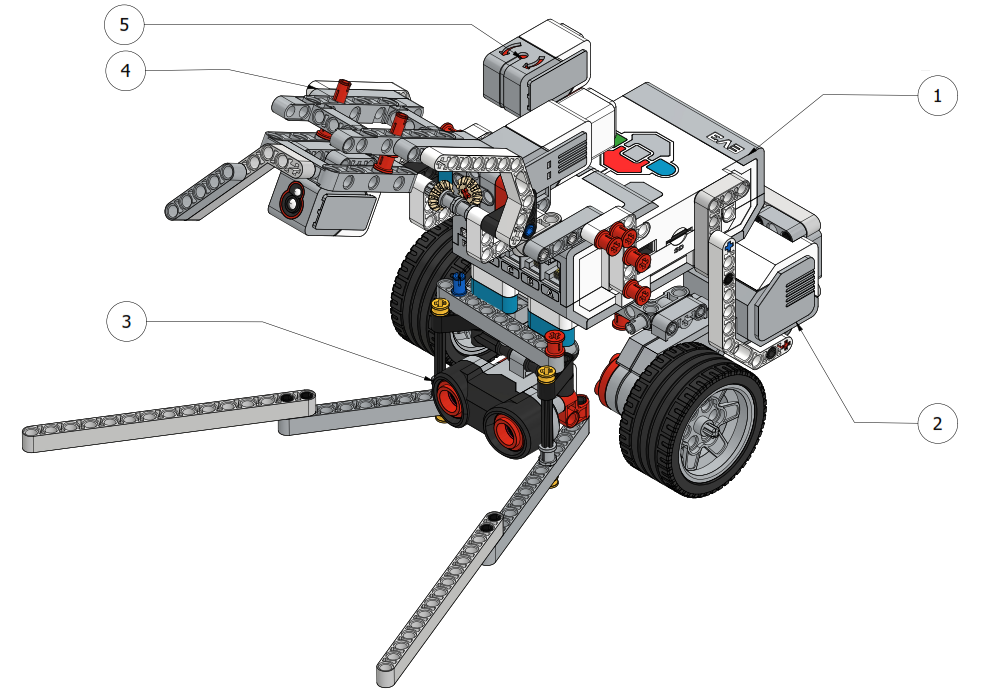
\includegraphics[width=0.8\linewidth]{Graphics/LabelledFruta}
	\caption{Main Components of Fruta Oes}
	\label{fig:labelledfruta}
\end{figure}

\noindent The five main components of this robot are listed in \vref{tab:mechanicalComponents}. \textbf{Item 1-EV3 Brick} is the heart and brain of the robot, the processing of the software takes place in this module. \textbf{Item 2-Drive Base} serves two purposes; providing stability and mobility, the in-depth design of this module will be discussed in \vref{sec:DriveBase}.

	\begin{table}[!ht]
	\centering
	\caption{Main Components}
	\vspace{-2mm}
	\label{tab:mechanicalComponents}
		\begin{tabular}{cl}
			\hline
			\textbf{Item}&\textbf{Component}\\
			\hline
			1&EV3 Brick\\
			2&Drive Base\\
			3&Object Detection and Manipulator Module\\
			4&Gripper and Colour Sensing Module\\
			5&Gyro-Sensor\\
			\hline			
		\end{tabular}
\end{table}

\noindent \textbf{Item 3-Object Detection and Manipulator Module} not only enable object detection capabilities but also makes sure that the object is manipulated to be in a good position for the gripping action. Object Detection and Manipulator Module will be fully discussed in \vref{sec:ObjectDetectionAndHandling}. \textbf{Item 4-Gripper and Colour Sensing Module} grips the object and makes sure it is in a good position for the colour sensor.
\noindent 
\subsection{Object Detection and Manipulator Module}\label{sec:ObjectDetectionAndHandling}

\noindent This section discusses the object detection mechanism. This module not only enable object detection capabilities but also makes sure that the object is manipulated to be in a good position for the gripping action. 
\begin{figure}[!ht]
	\centering
	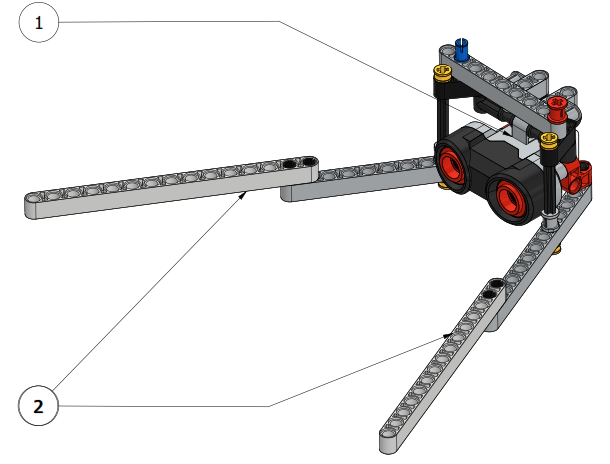
\includegraphics[width=0.8\linewidth]{Graphics/ObjectDetection}
	\caption{Object Detection and Manipulator Module}
	\label{fig:objectDetection}
	\vspace{-5mm}
\end{figure}

\begin{table}[!ht]
	\centering
	\caption{Object Detection and Manipulator Module Components}
	\vspace{-2mm}
	\label{tab:ObjectDetectionComponents}
	\begin{tabular}{cl}
		\hline
		\textbf{Item}&\textbf{Component}\\
		\hline
		1&Ultra Sonic Sensor\\
		2&Manipulator Fangs\\
		\hline			
	\end{tabular}
\end{table}

\noindent \Vref{fig:objectDetection} shows the object detecting manipulator, it is composed of two main parts listed in \vref{tab:ObjectDetectionComponents}: the ultrasonic Sensor which enables the fruit detection capability for the robot and the manipulator fangs. The ultra-sonic sensor is positioned as low as possible, because the objects to be detected are of 2.5cm height. This sensor is also used to provide distances to the robot as it is also capable of computing the distance to the detected object. The EV3 sensor has a measuring range of 250 cm and an accuracy range of $\pm$ 1cm. During the testing phase of the sensors, it was noted that the sensor is sometimes losing the object when the robot is approaching the detected object, this lead to the introduction of the manipulator fangs which are just LEGO beams positioned in such a way that they manipulate the object to slide and ends up in-front of the sensor. This mechanism improved the object detection and made the gripping operation and colour sensing easier. The latter will be discussed later in the document.
\vspace{-5mm}
\subsection{Gripper and Colour Sensing Module}\label{sec:Gripper}

\noindent This section presents the design of the colour sensing and gripping mechanism. This module is also equipped with manipulating fangs. This module is designed to with two states, opened and closed, the module must be fully opened during the searching of fruits in the acre to avoid distracting the signal of the ultrasonic sensor module that was discussed in \vref{sec:ObjectDetectionAndHandling}.
\begin{figure}[!ht]
	\centering
	\begin{subfigure}[b]{0.45\textwidth}
		\centering
		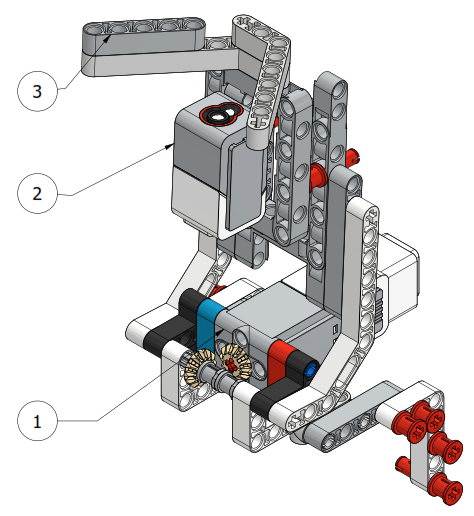
\includegraphics[width=\textwidth]{Graphics/OpenedGripper}
		\caption{Opened Gripper}
		\label{fig:OpenedGripper}
	\end{subfigure}
	~
	\begin{subfigure}[b]{0.45\textwidth}
		\centering
		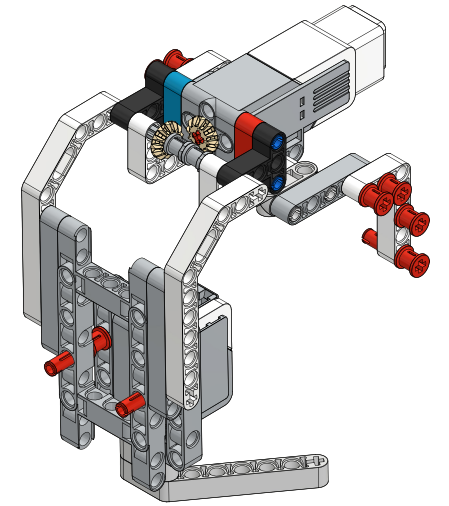
\includegraphics[width=\textwidth]{Graphics/ClosedGripper}
		\caption{Closed Gripper}
		\label{fig:ClosedGripper}
	\end{subfigure}
	\caption{Gripper and Colour Sensing Module}
	\vspace{-4mm}
	\label{fig:gripper}
\end{figure}

\begin{table}[!ht]
	\centering
	\caption{Gripper and Colour Sensing Module Components}
	\vspace{-2mm}
	\label{tab:ColourSensingComponents}
	\begin{tabular}{cl}
		\hline
		\textbf{Item}&\textbf{Component}\\
		\hline
		1&EV3 medium servo motor\\
		2&EV3 Colour Sensor\\
		3&Gripper Manipulator fangs\\
		\hline			
	\end{tabular}
\end{table}


\noindent \Vref{fig:gripper} depicts te gripper and the colour sensing module. \vref{fig:OpenedGripper} shows the gripper in opened mode and \vref{fig:ClosedGripper} shows the gripper in closed mode. This module comprises of three major components: EV3 medium servo motor, this motor is a great solution when the design of the robot requires shorter response times like the harvesting robot designed in this project. The motor is used for opening and closing mechanism of the gripper, it is equipped with 240 to 250 rpm and 0.08 Nm of running torque. The next component is an EV3 Colour sensor, the main function of this component is to enable the robot to distinguish between the required fruits and non-required fruits. The EV3 Colour Sensor is capable of detecting seven colours plus the absence of colour. It can tell the difference between colour or black-and-white or among blue, green, yellow, red, white, and brown. This sensor samples at a rate of 1 kHz, it must be positioned 1cm away from the object for better results.

\subsection{Drive Base}\label{sec:DriveBase}

\noindent In this section, the assembling of the drive base for the robot is discussed. it is made up of two parts: EV3 large motors and the wheels, also listed in \vref{tab:DriveBaseComponents}. there is also a balancing wheel positioned underneath the base close to the rear but this wheel is not shown in \vref{fig:DriveBase}.

\begin{figure}[!ht]
	\centering
	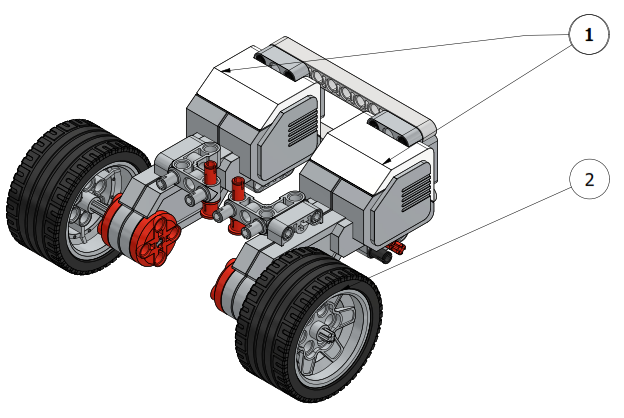
\includegraphics[width=\linewidth]{Graphics/DriveBase}
	\caption{Drive Base}
	\label{fig:DriveBase}
\end{figure}

\begin{table}[!ht]
	\centering
	\caption{Drive Base Components}
	\vspace{-2mm}
	\label{tab:DriveBaseComponents}
	\begin{tabular}{cl}
		\hline
		\textbf{Item}&\textbf{Component}\\
		\hline
		1&EV3 Large Motors\\
		2&Wheels\\
		\hline			
	\end{tabular}
\end{table}

\noindent The EV3 Large Servo Motor uses tacho feedback for accurate control to within one degree. The intelligent motor may be coordinated with other robot motors to move in a straight line at the same speed by using the built-in rotation sensor. This motor has an angular velocity ($\omega$) of 160 - 170 rpm, and can produce a running torque of 20 $N.cm$ and a stall torque of 40 $N.cm$ \cite{raisingRobots}. In the design of this drive base, each EV3 large motor is coupled with a 56 $milimeter$ diameter wheel. The dimensions of these wheels will become handy later when developing an algorithm to move the robot from one point to another for a specified distance. Appendix E shows a python function where a circumference of the wheels is used to move the robot forward and backwards, this function will be explain in depth in \vref{sec:softwareDesign}.

\newpage
\section{Software Design}\label{sec:softwareDesign}

\subsection{Task Solution}\label{sectaskSolution}
\noindent A solution to harvesting specific fruit uses mainly the ultrasonic sensor for searching for objects in an area. The solution that will be presented in this software design requires one to understand terms used for sectioning the field.  \Vref{fig:fruitScanning} shows the field, the field consists of a part called \textbf{Acre}, this part will have a mixture of fruits, required fruits and the non-required fruits. There is a \textbf{Main Line}, this is the line that will be used to track the movement of the robot, the robot will have to return to this line after every task it completes. Then there is \textbf{Home-Zone} where required fruits will be delivered to from the \textbf{Acre}.\\
~\\
\noindent \Vref{fig:turning90left} shows the robot in a starting position, the blue and orange lines from the robot illustrates the ultrasonic sound, the distance that is searched is also determined. The robot must turn left 90 degrees at a slow speed and determine is there are objects in the specified range (the robot pose after this turn is shown in \Vref{fig:turning90right}), then for assurance, the robot searched again by turning right 90 degrees and pose parallel to the main line.\\
\noindent After a complete scan, the robot advances by a short distance, and do the similar search until it detects an object after which the object is approached (\vref{fig:objectApproached}). The robot places the approached fruit under the colour sensor to determine if it is the desired fruit or not. If the fruit is not desired, the robot then pushes the fruit out of the way and then return to the main line to search again as shown in \vref{fig:objectPushed}. When a desired fruit is found (in this example a green object in \vref{fig:objectDelivered}), the robot pushes the fruit to the home zone and return to the main line until two fruits are harvested.
\begin{figure}[!ht]
	\centering
	\begin{subfigure}[b]{0.45\textwidth}
		\centering
		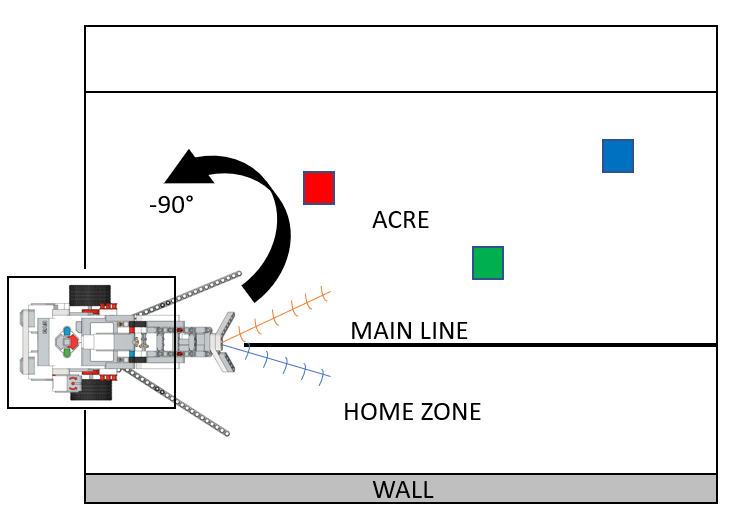
\includegraphics[width=\textwidth]{Graphics/turning90left}
		\caption{Robot Starting Position}
		\label{fig:turning90left}
	\end{subfigure}
	~
	\begin{subfigure}[b]{0.45\textwidth}
		\centering
		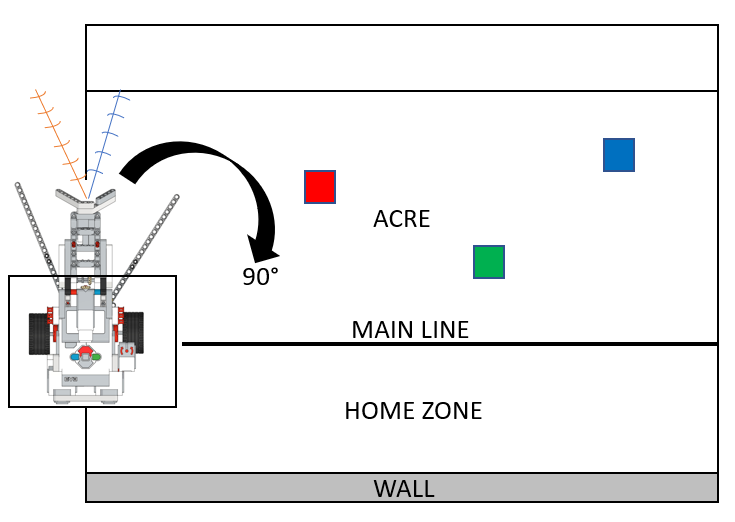
\includegraphics[width=\textwidth]{Graphics/turning90right}
		\caption{Position after 1 scan}
		\label{fig:turning90right}
	\end{subfigure}
	\caption{Fruit Searching}
	\vspace{-4mm}
	\label{fig:fruitScanning}
\end{figure}

\begin{figure}[!ht]
	\centering
	\begin{subfigure}[b]{0.45\textwidth}
		\centering
		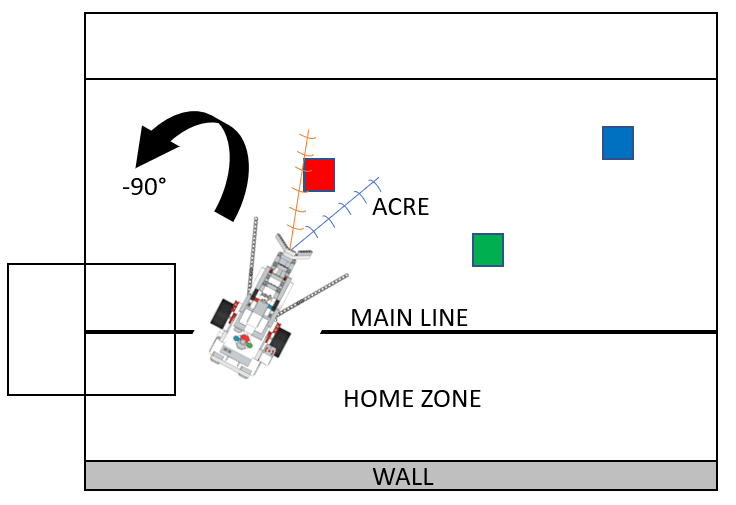
\includegraphics[width=\textwidth]{Graphics/objectDetected}
		\caption{Object Detected}
		\label{fig:objectDetected}
	\end{subfigure}
	~
	\begin{subfigure}[b]{0.45\textwidth}
		\centering
		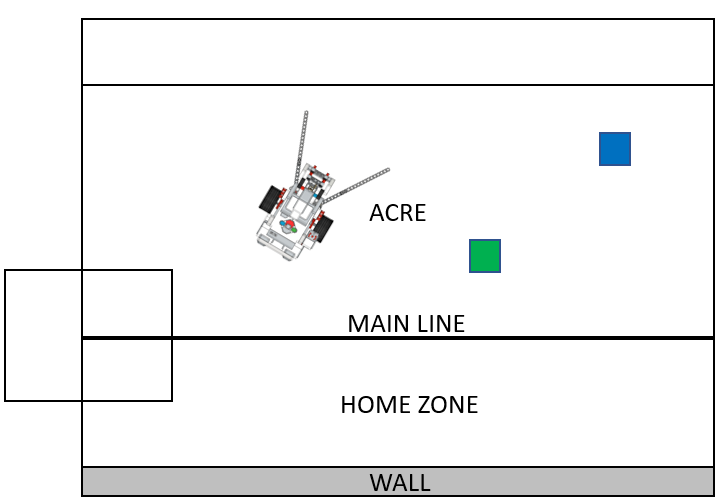
\includegraphics[width=\textwidth]{Graphics/objectApproached}
		\caption{Object Approached}
		\label{fig:objectApproached}
	\end{subfigure}
	\caption{Fruit Searching in new position}
	\label{fig:fruitScanning2}
	\vspace{-4mm}
\end{figure}

\begin{figure}[!ht]
	\centering
	\begin{subfigure}[b]{0.45\textwidth}
		\centering
		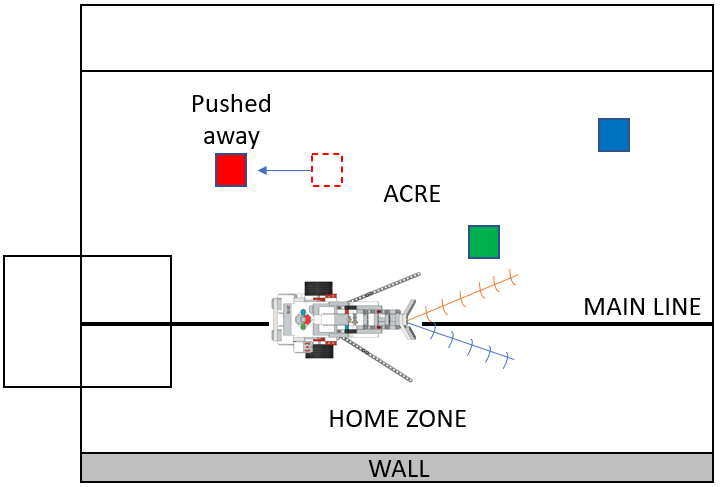
\includegraphics[width=\textwidth]{Graphics/objectPushed}
		\caption{Object Detected}
		\label{fig:objectPushed}
	\end{subfigure}
	~
	\begin{subfigure}[b]{0.45\textwidth}
		\centering
		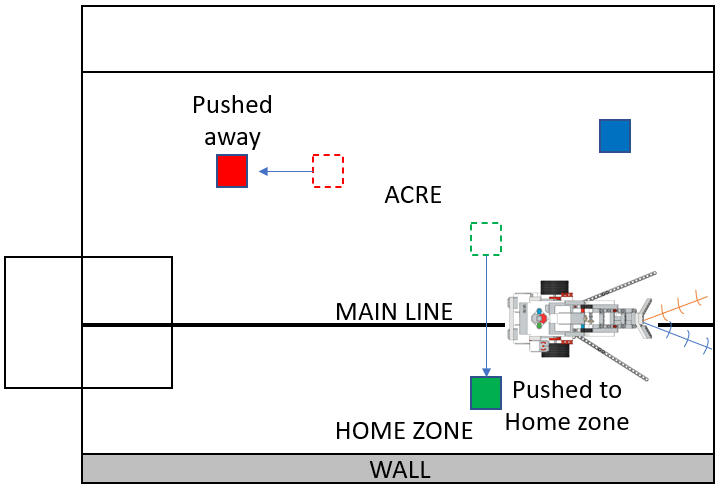
\includegraphics[width=\textwidth]{Graphics/objectDelivered}
		\caption{Object Approached}
		\label{fig:objectDelivered}
	\end{subfigure}
	\caption{Undesired and desired fruit}
	\label{fig:fruitSensing}
	\vspace{-4mm}
\end{figure}


\newpage
\subsection{Main Code}\label{sec:mainCode}

\noindent This section discusses the execution of the main function. \Vref{fig:MainCodeActivityDiagram} presents the activity diagram for this main function. Firstly, Python need libraries are imported (e.g EV3 library, Math library, EV3 brick buttons library, Time library). This function deploys the robot to harvest fruits and only returns to the starting position if one of the two conditions is met: 1. if the robot harvested two fruits it must then return. 2. if a five minute times out while searching, the robot must return home. A safety condition to make sure the robot does not exceed the limits of the field was implemented. If the robot moved a distance of four minutes along the main line without finding fruits, it is then sent back to the starting position to do the search once again.
\begin{figure}[!ht]
	\centering
	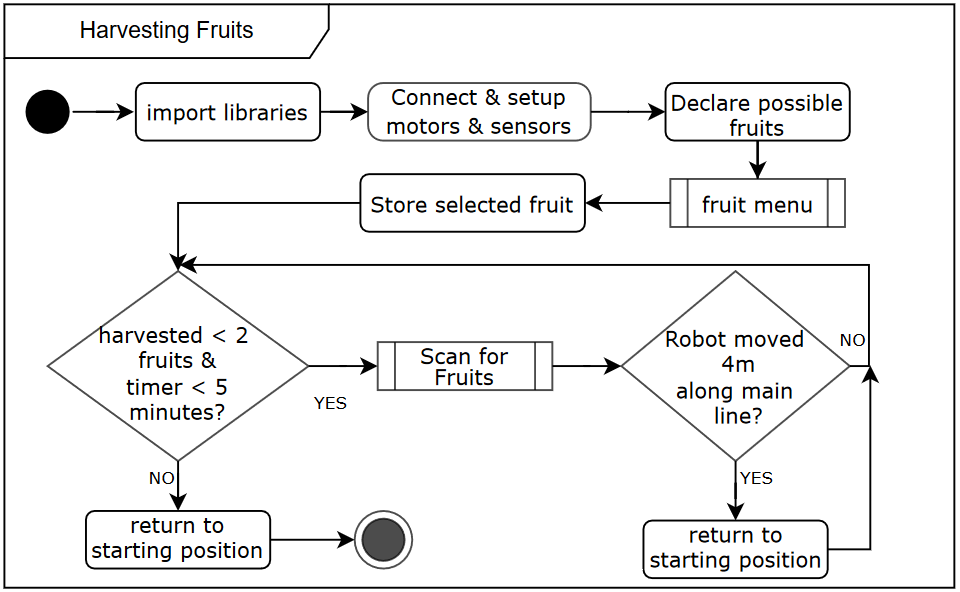
\includegraphics[width=\linewidth]{Graphics/mainCodeActivityDiagram3}
	\caption{Main Code Activity Diagram}
	\label{fig:MainCodeActivityDiagram}
\end{figure}

\vspace{-5mm}

\begin{algorithm}
	\caption{: Main Function Pseudo Code}\label{mainPseudo}
	\begin{algorithmic}[1]
		\State Import libraries and connect devices;
		\State Create a fruit dictionary with 4 fruits and 4 buttons;
		\State Call fruit menu() function and store the selected fruit;
		\While{harvested < 2 fruits and timer < 5 minutes}
		\State Call scanning() function;
			\If{Robot reached the end of the main line (4m)?}
				\State Return to the starting position;
			\EndIf
		\EndWhile
		\State Return to the starting position;
	\end{algorithmic}
\end{algorithm}

\newpage
\subsection{User Menu for Selecting the Colour (fruit)}\label{sec:menuCode}

\noindent As it can be seen in \vref{fig:2oppositeviews}, the EV3 brick buttons are coloured with all possible colours of the project: Left button for Blue, Up button for Red and right button for green. The user must wait for the beep after the robot asked them to select the colour from the buttons. Based on the pressed button, the robot will confirm the chosen colour and proceed to search for that specific fruit in the acre. \Vref{fig:menuCodeActivityDiagram} presents the activity diagram for User Menu function, the corresponding source code is attached on appendix B.

\begin{figure}[!ht]
	\centering
	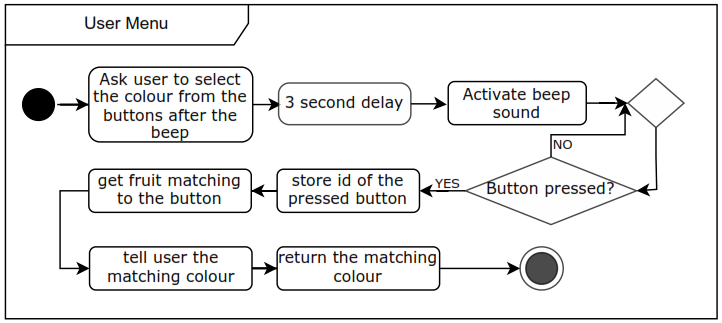
\includegraphics[width=\linewidth]{Graphics/menuCodeActivityDiagram}
	\caption{Menu Code Activity Diagram}
	\label{fig:menuCodeActivityDiagram}
\end{figure}
\vspace{-3mm}
\noindent \Vref{menuPseudo} presents a pseudo code for this user menu method. A five minute timer is started at the beginning of the function, because one of the requirements is that the robot must return to the starting position after five minutes and this time must be measured as soon as the robot starts interacting with the user. This algorithm is constructed from the activity diagram above.

\begin{algorithm}
	\caption{: User Menu Method Pseudo Code}\label{menuPseudo}
	\begin{algorithmic}[1]
		\State Start the 5 minutes timer;
		\State Use EV3 Speaker function to ask the user to select the colour from the buttons after the beep;
		\State sleep for 3 seconds to allow the sound command to complete;
		\State Activate the EV3 Beep Sound;
		\While{\textit{True}}
		\If{Any button is pressed}
		\State Store the id of the pressed button;
		\State break out of the while loop;
		\EndIf
		\EndWhile
		\State Use the id of the pressed button to get matching fruit from the fruit dictionary;
		\State Use EV3 speaker to tell the user the matching colour;
		\State Return the matching colour to the rest of the code;
	\end{algorithmic}
\end{algorithm}

\newpage
\subsection{Driving from Acre to Main line and Home Zone}
\noindent The position and orientation of the robot needed to be tracked to be sure that it drives to correct areas of the field. This was obtained by using trigonometry functions (\vref{eq:1}). \Vref{fig:drivingtoMLHZ} shows the graphical analysis. The angle at which the object is detected is saved, also the distance the robot travelled to the object(hypotenuse). What is left is to find the opposite distance(d) of the triangle. For driving to the main line, the robot must drive the distance (d) (\vref{fig:drivingtoML}) and to drive to the home zone, 20 cm are added to this distance (\vref{fig:drivingtoHZ}).


\begin{equation}
	opposite(d) = hypotenuse(r) \times \sin \theta \label{eq:1}
\end{equation}

\begin{figure}[!ht]
	\centering
	\begin{subfigure}[b]{0.45\textwidth}
		\centering
		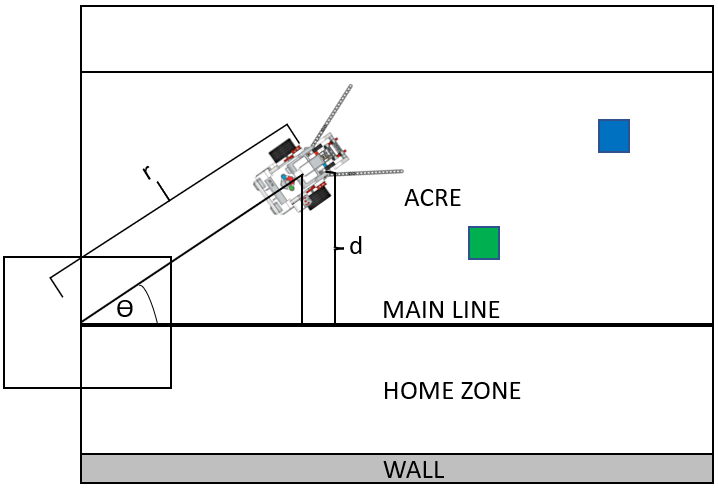
\includegraphics[width=\textwidth]{Graphics/acreToML}
		\caption{Driving from Acre to Main line}
		\label{fig:drivingtoML}
	\end{subfigure}
	~
	\begin{subfigure}[b]{0.45\textwidth}
		\centering
		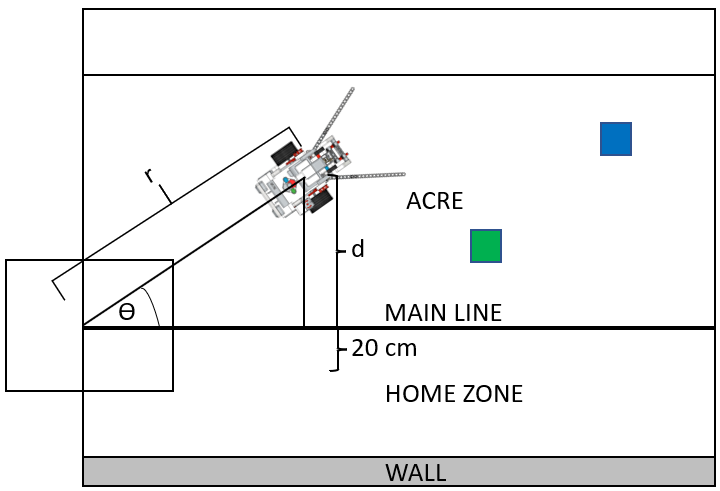
\includegraphics[width=\textwidth]{Graphics/acreToHZ}
		\caption{Driving from Acre to home zone}
		\label{fig:drivingtoHZ}
	\end{subfigure}
	\caption{Driving from Acre to Main line and Home zone}
	\label{fig:drivingtoMLHZ}
	\vspace{-4mm}
\end{figure}

\subsection{Scanning Function and Ultra-Sonic Sensor Optimization}
\noindent The activity diagram for the scanning function is shown in \vref{fig:scaddingActivityDiagram}. This function makes use of the following algorithm to pin point the exact point of the object. The robot finds the edges of the object (\cref{fig:opt1} and \cref{fig:op2}) and calculates the centre angle as shown in \cref{fig:opt3}.
\begin{figure}[!ht]
	\centering
	\begin{subfigure}[b]{0.3\textwidth}
		\centering
		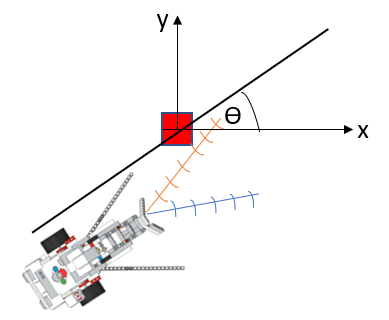
\includegraphics[width=\textwidth]{Graphics/opt1}
		\caption{first Edge of object}
		\label{fig:opt1}
	\end{subfigure}
	~
	\begin{subfigure}[b]{0.3\textwidth}
		\centering
		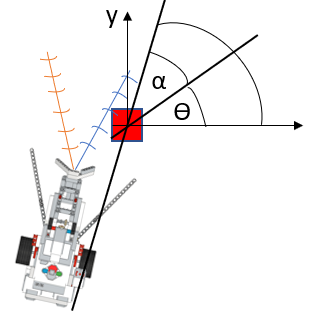
\includegraphics[width=\textwidth]{Graphics/opt2}
		\caption{Second Edge of object}
		\label{fig:op2}
	\end{subfigure}
	~
	\begin{subfigure}[b]{0.3\textwidth}
	\centering
	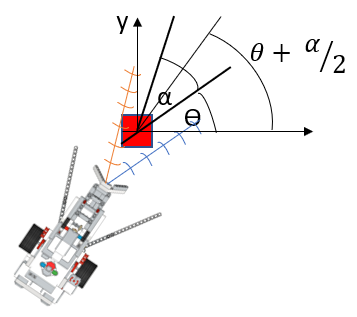
\includegraphics[width=\textwidth]{Graphics/opt3}
	\caption{Optimized angle}
	\label{fig:opt3}
	\end{subfigure}
	\caption{Ultra-Sonic Sensor Optimization}
	\label{fig:optimization}
	\vspace{-4mm}
\end{figure}


\begin{figure}[!ht]
	\centering
	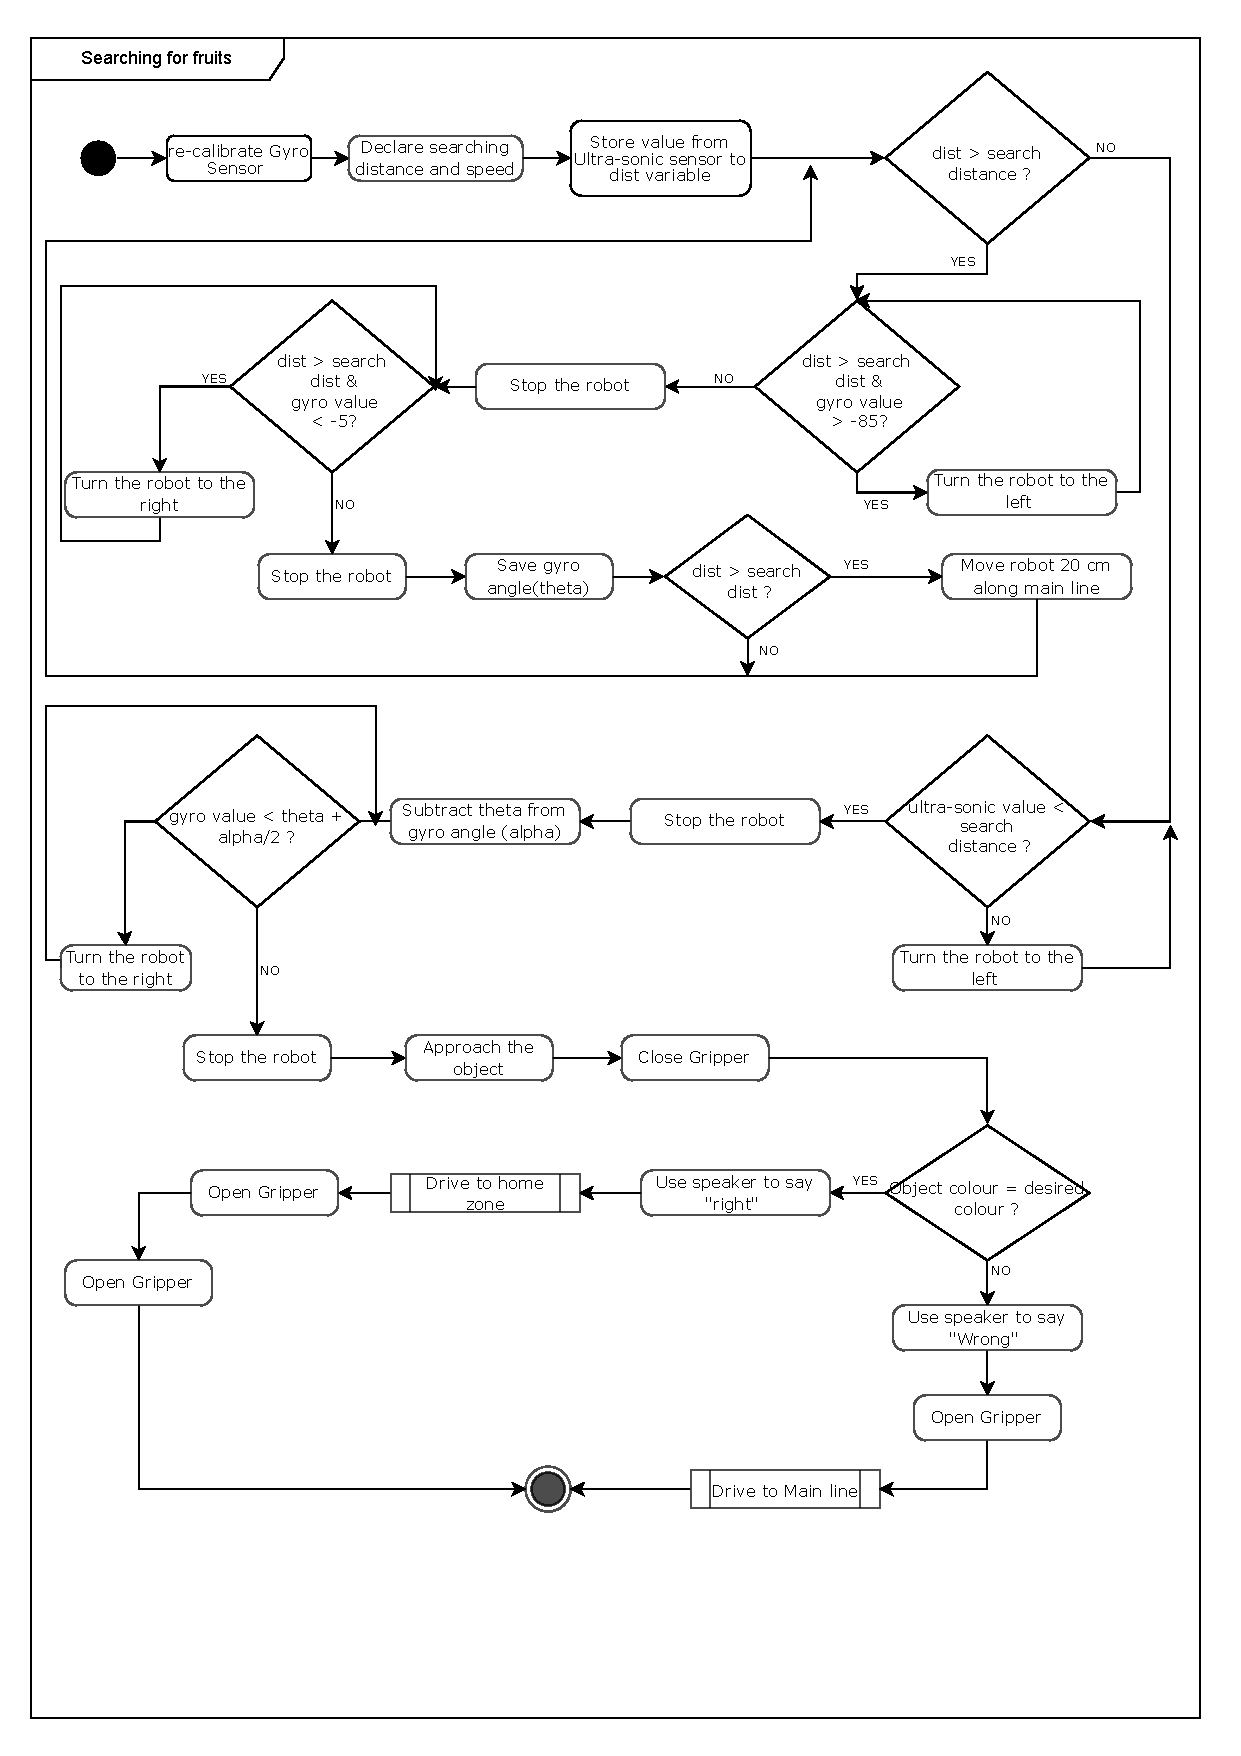
\includegraphics[width=0.95\linewidth]{export-1.pdf}
	\vspace{-4mm}
	\caption{Scanning Code Activity Diagram.}
	\label{fig:scaddingActivityDiagram}
\end{figure}
\newpage
\section{Analysis: Plan how to tackle the problem}\label{sec:softwareEngineering}
\subsection{Project Setup} \label{sec:projectSetup}
\noindent This section presents the project setup. The project vision is pitched in this section, the Scrum team is introduced, and the product backlog is presented.
\begin{comment}
	\noindent LEF BOTS GmbH is a robot specialising company, the name of the firm is created from the initials of the stakeholders: \textbf{L}aura; \textbf{E}ncarnacion; \textbf{F}erlando \textbf{(LEF)}. In this text, the firm presents the development of its major product; the fruit harvesting robot. The robot is given an intuitive name \textbf{Fruta Oes}, which is a combination of two languages Spanish and Afrikaans. Fruta means fruits in Spanish and Oes means to harvest in Afrikaans, thus, the name of the robot \textbf{Fruta Oes} means fruits harvester. One might be asking themselves why Spanish and Afrikaans, well the answer is simple, the stakeholders of the firm are from Spain (Laura and Encarnacion) and South Africa (Ferlando). \Vref{fig:2oppositeviews} Presents \textbf{Fruta Oes}. ...
\end{comment}


\subsubsection{Project Vision}

"For harvesters who care for the environment. We believe in a world where harvesters can harvest being eco-friendly" 


\subsubsection{SCRUM Team}
\noindent \Vref{fig:scrumTeam} presents the scrum team: Encarnacion Nunez-Ortega is the \textbf{Product Owner} and responsible for determining what needs to be done. Laura Ponce-Orozco is the team's \textbf{Scrum master} and responsible for removing all impediments. The \textbf{development team} consist of Ferlando Mkiva, Encarnacion Nunez-Ortega and Ponce-Orozco together will determine how to deliver chunks of work in frequent increments.
\begin{figure}[!ht]
	\centering
	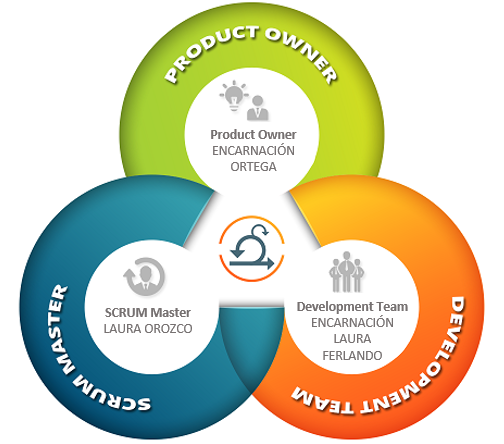
\includegraphics[width=0.6\linewidth]{Graphics/scrumTeam}
	\caption{SCRUM Team}
	\label{fig:scrumTeam}
\end{figure}

\newpage
\subsubsection{Product Backlog}\label{sec:projectBacklog}

\noindent \Vref{tab:productBacklog} Present the Product backlog for the project. This table comprises ordered list of user stories that have been derived from the requirements. In other words, all the features of the product that is designed in this project are listed in this table. The first column shows the priority of the user stories from 1-10, priority 1 means it is the most important task. 
\begin{table}[!ht]
	\centering
	\caption{Product Backlog}
	\label{tab:productBacklog}
	\begin{tabular}{c p{30.645em} c}
		\toprule
		\textbf{Priority}&\multicolumn{1}{l}{\textbf{User Story}} & \textbf{Effort} \\
		\midrule
		1&As a user, I want the robot to be completely autonomous. & \adjustimage{height=0.6cm,valign=m}{Graphics/effort1} \\
		\midrule
		2&As a user, I want the robot to ask me for the correct fruit and to confirm that it understood me. & \adjustimage{height=0.6cm,valign=m}{Graphics/effort2} \\
		\midrule
		3&As a developer, I want the robot to be able to detect a 2.5cm cube. & \adjustimage{height=0.6cm,valign=m}{Graphics/effort1} \\
		\midrule
		4&As a user, I want the robot to look for the specified fruit and check if the fruit is correctly grabbed. & \adjustimage{height=0.6cm,valign=m}{Graphics/effort5}\\
		\midrule
		5&As a user, I don’t want the robot to return to the home zone without the fruit grabbed. & \adjustimage{height=0.6cm,valign=m}{Graphics/effort4} \\
		\midrule
		6&As a user, I want the robot to place the right fruit in the home zone. & \adjustimage{height=0.6cm,valign=m}{Graphics/effort3} \\
		\midrule
		7&As a developer, I want the robot to keep count of the harvested fruits & \adjustimage{height=0.6cm,valign=m}{Graphics/effort1} \\
		\midrule
		8&As a user, I want the robot to immediately return to the starting point after collecting two fruits within 5 minutes. & \adjustimage{height=0.6cm,valign=m}{Graphics/effort4} \\
		\midrule
		9&As a user, I don’t want the robot to search for fruits outside the acre. & \adjustimage{height=0.6cm,valign=m}{Graphics/effort3} \\
		\midrule
		10&As a developer, I want the code to be efficient.  & \adjustimage{height=0.6cm,valign=m}{Graphics/effort4} \\
		\bottomrule
	\end{tabular}%
\end{table}%


\subsection{Sprint 1} \label{sec:sprint1}
\subsubsection{Goals of the sprint}\label{sec:sprint1goals}
\noindent The goal of this sprint was to tackle the following user stories. In total eight cups of coffees must be consumed as the effort of this sprint.\\
~\\
\begin{minipage}[t]{0.35\textwidth}
	\begin{StickyNote}
		As a \textbf{user}, I want the robot to ask me for the \textbf{correct fruit} and to confirm that it understood me.
		\adjustimage{height=0.6cm,valign=m}{Graphics/effort22}
	\end{StickyNote}
\end{minipage}
\begin{minipage}[t]{0.3\textwidth}
		\begin{StickyNote}
		As a \textbf{developer}, I want the robot to be able to \textbf{detect} a 2.5cm cube.
		\adjustimage{height=0.6cm,valign=m}{Graphics/effort12}
	\end{StickyNote}
\end{minipage}
\begin{minipage}[t]{0.35\textwidth}
	\begin{StickyNote}
	As a \textbf{user}, I want the robot to look for the \textbf{specified fruit} and check if the fruit is correctly grabbed.
	\adjustimage{height=0.6cm,valign=m}{Graphics/effort52}
\end{StickyNote}
\end{minipage}



\subsubsection{Burn-down Chart}\label{sec:sprint1bdc}
\begin{figure}[H]
	\centering
	\begin{tikzpicture}
		\begin{axis}
			[
			legend pos=north east,
			every axis plot/.append style={ultra thick},
			xmin = 0,
			ymin = 0,
			xmajorgrids=true,
			grid style=dashed,
			width=0.8\textwidth,
			height=0.5\textwidth,
			xlabel=\textbf{Days},
			ylabel=\textbf{Coffees \adjustimage{height=0.6cm,valign=m}{Graphics/effortN}},
			y tick label style={
				/pgf/number format/.cd,
				fixed,
				fixed zerofill,
				precision=0,
				/tikz/.cd
			},
			x tick label style={
				/pgf/number format/.cd,
				fixed,
				fixed zerofill,
				precision=0,
				/tikz/.cd
			},
			scaled ticks=false,
			yticklabel={${\pgfmathprintnumber{\tick}}$},
			]
			\addlegendimage{empty legend}
			\addplot[orange, mark=none] table[x index=0, y index=1, col sep=comma] {Sprint1.csv};
			\addplot[green, mark=none] table[x index=2, y index=3, col sep=comma] {Sprint1.csv};
			\addlegendentry{\hspace{-.6cm}\textbf{Burn-down Charts}}
			\addlegendentry{Actual}
			\addlegendentry{Ideal}
		\end{axis}
	\end{tikzpicture}
	\vspace{-1mm}
	\caption{Sprint 1 Burn-down Chart}
	\label{fig:sprint1BurndownChart}
\end{figure}

\noindent The increment of this Sprint was 4 instead of 8 coffees in view of the fact that we underestimated the tasks. We have an incomplete user story which states: As a user, I want the robot to look for the specified fruit and check if the fruit is correctly grabbed. This user story was deemed incomplete as the robot's capabilities were limited to searching for any fruit and not a specific one, as well as the inability to properly grasp the fruit. As a result, we had to add 4 extra story points to the next Sprint and address the incomplete user story during the next Sprint Planning.

\subsection{Test: expected and actual results, bug fixing.}

\textbf{User Story:} \emph{As a user, I want the robot to ask me for the correct fruit and to confirm that it under- stood me.}\\~\\
\noindent We initially attempted to identify the colour of the fruit using a colour sensor and showing directly the cube, but it proved to be unreliable as it also picked up the colour of the floor. To address this, we limited the sensor to only detect blue, green, and red. However, this caused confusion when distinguishing between red and green. To improve accuracy, we implemented a manual method, using buttons on the brick to identify the colour. 
\newpage
\subsection{Sprint 2}	\label{sec:sprint2}

\subsubsection{Goals of the sprint}\label{sec:sprint2goals}
\noindent The goal of this sprint was to tackle the following user stories. In total twelve cups of coffees must be consumed as the effort of this sprint.\\
~\\
\begin{minipage}[t]{0.23\textwidth}
	\begin{StickyNote}
		As a \textbf{user}, I want the robot to place the \textbf{right fruit} in the home zone.
		\adjustimage{height=0.6cm,valign=m}{Graphics/effort32}
	\end{StickyNote}
\end{minipage}
\begin{minipage}[t]{0.24\textwidth}
	\begin{StickyNote}
		As a \textbf{user}, I don’t want the robot to \textbf{return} to the home zone \textbf{without the fruit} grabbed.
		\adjustimage{height=0.6cm,valign=m}{Graphics/effort42}
	\end{StickyNote}
\end{minipage}
\begin{minipage}[t]{0.26\textwidth}
	\begin{StickyNote}
		As a \textbf{user}, I want the robot to look for the \textbf{specified fruit} and check if the fruit is correctly grabbed.
		\adjustimage{height=0.6cm,valign=m}{Graphics/effort52}
	\end{StickyNote}
\end{minipage}
\begin{minipage}[t]{0.22\textwidth}
	\begin{StickyNote}
		As a \textbf{user}, I want the robot to be completely \textbf{autonomous}.
		\adjustimage{height=0.6cm,valign=m}{Graphics/effort12}
	\end{StickyNote}
\end{minipage}
\subsubsection{Burn-down Chart}\label{sec:sprint2bdc}
\begin{figure}[H]
	\centering
	\begin{tikzpicture}
		\begin{axis}
			[
			legend pos=north east,
			every axis plot/.append style={ultra thick},
			xmin = 0,
			ymin = 0,
			xmajorgrids=true,
			grid style=dashed,
			width=0.8\textwidth,
			height=0.5\textwidth,
			xlabel=\textbf{Days},
			ylabel=\textbf{Coffees \adjustimage{height=0.6cm,valign=m}{Graphics/effortN}},
			y tick label style={
				/pgf/number format/.cd,
				fixed,
				fixed zerofill,
				precision=0,
				/tikz/.cd
			},
			x tick label style={
				/pgf/number format/.cd,
				fixed,
				fixed zerofill,
				precision=0,
				/tikz/.cd
			},
			scaled ticks=false,
			yticklabel={${\pgfmathprintnumber{\tick}}$},
			]
			\addlegendimage{empty legend}
			\addplot[orange, mark=none] table[x index=0, y index=1, col sep=comma] {Sprint2.csv};
			\addplot[green, mark=none] table[x index=2, y index=3, col sep=comma] {Sprint2.csv};
			\addlegendentry{\hspace{-.6cm}\textbf{Burn-down Charts}}
			\addlegendentry{Actual}
			\addlegendentry{Ideal}
		\end{axis}
	\end{tikzpicture}
	\vspace{-1mm}
	\caption{Sprint 2 Burn-down Chart}
	\label{fig:sprint2BurndownChart}
\end{figure}

\noindent The increment of this Sprint was 11 instead of 12 coffees in view of the fact that we underestimated the tasks. We have an incomplete user story which states: As a user, I want the robot to be completely autonomous. This user story was deemed incomplete as the robot's brick did not detect the program correctly. As a result, we had to add 1 extra story point to the next Sprint and address the incomplete user story during the next Sprint Planning.

\subsubsection{Test: expected and actual results, bug fixing.}

\textbf{User Story:} \emph{As a user, I want the robot to look for the specified   fruit and check if the fruit is correctly grabbed.}\\
~\\
Initially, we aimed to calculate the angle at which we needed to rotate the robot in order to detect the specified fruit. To do this, we measured the detection range of the ultrasonic sensor by positioning a cube at varying distances and marking the points at which the sensor first detected the cube. We then calculated the center of this detection range as a point of reference for approaching the fruit. However, we found that this method was not consistently accurate as the detection range varied. As an alternative, we decided to rotate the robot to the left by 90 degrees and then save the angle at which the fruit was first detected (see \vref{sec:softwareDesign}). Through testing with various positions of the fruit, we determined that this approach was the most effective.

\subsubsection{Product Backlog}
\begin{minipage}[t]{0.35\textwidth}
	\centering
	\textbf{Open} \adjustimage{height=0.6cm,valign=m}{Graphics/effort122}
	\begin{StickyNote}
	As a \textbf{developer}, I want the robot to \textbf{keep count} of the harvested fruits.
	\adjustimage{height=0.6cm,valign=m}{Graphics/effort12}
	\end{StickyNote}
	\begin{StickyNote}
	As a \textbf{user}, I want the robot to immediately \textbf{return} to the \textbf{starting point} after collecting 2 fruits within 5 minutes.
	\adjustimage{height=0.6cm,valign=m}{Graphics/effort42}
	\end{StickyNote}
	\begin{StickyNote}
	As a \textbf{user}, I do not want the robot to search for fruits  \textbf{outside} the \textbf{acre}.
	\adjustimage{height=0.6cm,valign=m}{Graphics/effort32}
	\end{StickyNote}
	\begin{StickyNote}
		As a \textbf{developer}, I want the the code to be \textbf{efficient}.
		\adjustimage{height=0.6cm,valign=m}{Graphics/effort42}
	\end{StickyNote}
\end{minipage}
{\vrule width 2pt}
\begin{minipage}[t]{0.3\textwidth}
	\centering
	\textbf{Doing} \adjustimage{height=0.6cm,valign=m}{Graphics/effort12}
	\begin{BStkyNote}
	As a \textbf{user}, I want the robot to be completely \textbf{autonomous}.
	\adjustimage{height=0.6cm,valign=m}{Graphics/effort12}
	\end{BStkyNote}
\end{minipage}
{\vrule width 2pt}
\begin{minipage}[t]{0.35\textwidth}
	\centering
	\textbf{Done} \adjustimage{height=0.6cm,valign=m}{Graphics/effort152}
	\begin{GStkyNote}
		As a \textbf{user}, I don’t want the robot to \textbf{return} to the home zone \textbf{without the fruit} grabbed.
		\adjustimage{height=0.6cm,valign=m}{Graphics/effort42}
	\end{GStkyNote}
	\begin{GStkyNote}
		As a \textbf{user}, I want the robot to look for the \textbf{specified fruit} and check if the fruit is correctly grabbed.
		\adjustimage{height=0.6cm,valign=m}{Graphics/effort52}
	\end{GStkyNote}
	\begin{GStkyNote}
	As a \textbf{developer}, I want the robot to be able to \textbf{detect} a 2.5cm cube.
	\adjustimage{height=0.6cm,valign=m}{Graphics/effort12}
	\end{GStkyNote}
	\begin{GStkyNote}
	As a \textbf{user}, I want the robot to place the \textbf{right fruit} in the home zone.
	\adjustimage{height=0.6cm,valign=m}{Graphics/effort32}
	\end{GStkyNote}
	\begin{GStkyNote}
	As a \textbf{user}, I want the robot to ask me for the \textbf{correct fruit} and to confirm that it understood me.
	\adjustimage{height=0.6cm,valign=m}{Graphics/effort22}
	\end{GStkyNote}
\end{minipage}


\newpage
\subsection{Sprint 3} \label{sec:sprint3}
\subsubsection{Goals of the sprint}\label{sec:sprint3goals}

\noindent The goal of this sprint was to tackle the following user stories. In total thirteen cups of coffees must be consumed as the effort of this sprint.\\
~\\
\begin{minipage}[t]{0.23\textwidth}
	\begin{StickyNote}
		As a \textbf{developer}, I want the robot to \textbf{keep count} of the harvested fruits.
		\adjustimage{height=0.6cm,valign=m}{Graphics/effort12}
	\end{StickyNote}
\end{minipage}
\begin{minipage}[t]{0.33\textwidth}
	\begin{StickyNote}
		As a \textbf{user}, I want the robot to immediately \textbf{return} to the \textbf{starting point} after collecting 2 fruits within 5 minutes.
		\adjustimage{height=0.6cm,valign=m}{Graphics/effort42}
	\end{StickyNote}
\end{minipage}
\begin{minipage}[t]{0.24\textwidth}
	\begin{StickyNote}
		As a \textbf{user}, I do not want the robot to search for fruits  \textbf{outside} the \textbf{acre}.
		\adjustimage{height=0.6cm,valign=m}{Graphics/effort52}
	\end{StickyNote}
\end{minipage}
\begin{minipage}[t]{0.21\textwidth}
	\begin{StickyNote}
		As a \textbf{developer}, I want the the code to be \textbf{efficient}.
		\adjustimage{height=0.6cm,valign=m}{Graphics/effort42}
	\end{StickyNote}
\end{minipage}

\subsubsection{Burn-down Chart}\label{sec:sprint3bdc}
\begin{figure}[H]
	\centering
	\begin{tikzpicture}
		\begin{axis}
			[
			legend pos=north east,
			every axis plot/.append style={ultra thick},
			xmin = 0,
			ymin = 0,
			xmajorgrids=true,
			grid style=dashed,
			width=0.8\textwidth,
			height=0.5\textwidth,
			xlabel=\textbf{Days},
			ylabel=\textbf{Coffees \adjustimage{height=0.6cm,valign=m}{Graphics/effortN}},
			y tick label style={
				/pgf/number format/.cd,
				fixed,
				fixed zerofill,
				precision=0,
				/tikz/.cd
			},
			x tick label style={
				/pgf/number format/.cd,
				fixed,
				fixed zerofill,
				precision=0,
				/tikz/.cd
			},
			scaled ticks=false,
			yticklabel={${\pgfmathprintnumber{\tick}}$},
			]
			\addlegendimage{empty legend}
			\addplot[orange, mark=none] table[x index=0, y index=1, col sep=comma] {Sprint3.csv};
			\addplot[green, mark=none] table[x index=2, y index=3, col sep=comma] {Sprint3.csv};
			\addlegendentry{\hspace{-.6cm}\textbf{Burn-down Charts}}
			\addlegendentry{Actual}
			\addlegendentry{Ideal}
		\end{axis}
	\end{tikzpicture}
	\vspace{-1mm}
	\caption{Sprint 3 Burn-down Chart}
	\label{fig:sprint3BurndownChart}
\end{figure}

\noindent The increment of this Sprint was 11 instead of 13 coffees in view of the fact that we underestimated the tasks. We have an incomplete user story which states: As a developer, I want the code to be efficient. As a result, we spent the last week improving our code.

\subsubsection{Test: expected and actual results, bug fixing.}

\textbf{User Story:} \emph{As a developer, I want the robot to keep count of the harvested fruits.}\\~\\
To ensure the functionality of our code, we conducted multiple tests using varying quantities of fruits to be harvested. The results were satisfactory and the code performed as intended.
\newpage
\section{Discussion and reflection} \label{sec:RecommendationsAndConclusion}
\subsection{Results of the sprint retrospectives}
\noindent In regard to the first sprint retrospective, we identified utilizing a shared screen as a significant positive aspect as it allowed for greater efficiency and improved error detection through simultaneous code review. A negative aspect identified was the time wasted on experimenting with various approaches to the same task. We always continued implementing the highlights and discarding the lowlights in all following sprints.
For the second sprint retrospective, we recognized a positive aspect in that we learned about the working styles of each group member and were able to capitalize on that knowledge. On the negative side, we acknowledged that we spent a significant amount of time attempting to execute a specific approach, instead of exploring new ideas.
For the third sprint retrospective, we considered that thinking creatively and embracing new ideas was a highlight. However, the team's motivation was negatively impacted by a series of errors related to the sensors.

\subsection{Final discussion}
\noindent Using Scrum as a didactical method for this project has been a valuable and beneficial experience. Scrum is a widely used and well-established framework for Agile software development, and its principles and practices can be applied to a wide range of projects.
One of the advantages of using Scrum in this context is that it promotes active participation and collaboration among team members. The Scrum meetings, such as sprint planning, daily stand-ups, and retrospectives, provide opportunities for the team to communicate and work together effectively, which is crucial for a successful project. 
Furthermore, Scrum enables a focus on delivering value to the end-user through the use of user stories, which is a key aspect of the project, in this case, the end-user will be the farmer or the person who will use the harvesting robot.
In conclusion, working on a real-world project with Scrum has been a great opportunity to learn about Agile development and gain practical experience in project management, teamwork, and problem-solving, acquiring skills very useful for a student.

%\onehalfspacing
\bibliographystyle{plainnat}	
\bibliography{Main-pages/mybib}
~\\
\noindent Note: diagrams and graphs are works of the report authors. Specifically, drawings are created using Microsoft Visio Professional 2019 and Autodesk Inventor Student version 2023, algorithms are constructed using the \LaTeX~"algpseudocode" package, and Code appendices are constructed using the \LaTeX~"listings" package (with data obtained from Python). No work done by other persons is presented as that of the report author.

